\addcontentsline{toc}{chapter}{Appendix A: State-space}  
\section*{Appendix A: State-space}


% \begin{figure}[ht]
    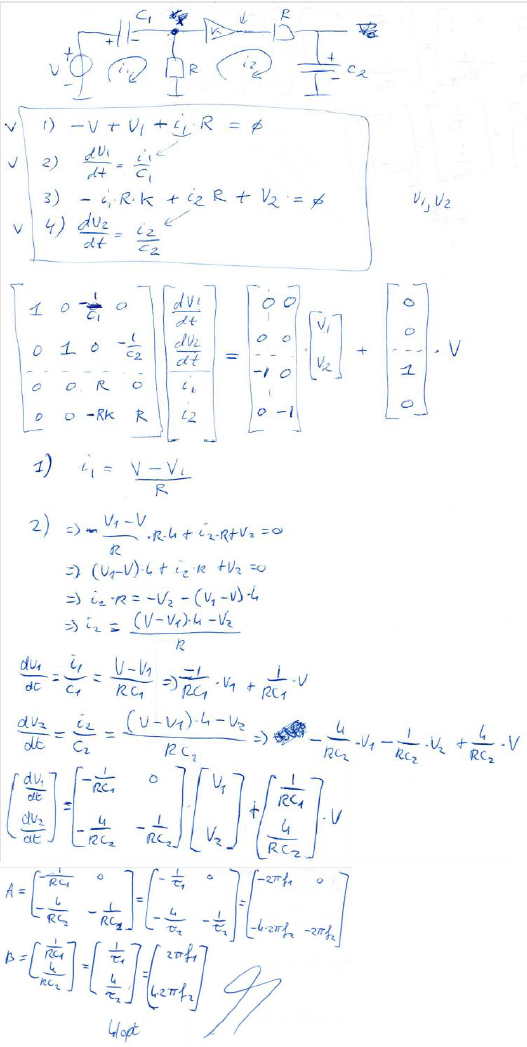
\includegraphics[width=\linewidth, height=\textheight, keepaspectratio]{State-space_notation_solution.png}
    \caption{State-space notation derived from band-pass filter circuit}
%     \label{fig:state-space-derived-bpf}
% \end{figure}
\newpage
\newpage

\section*{Appendix B: Main board schematic}
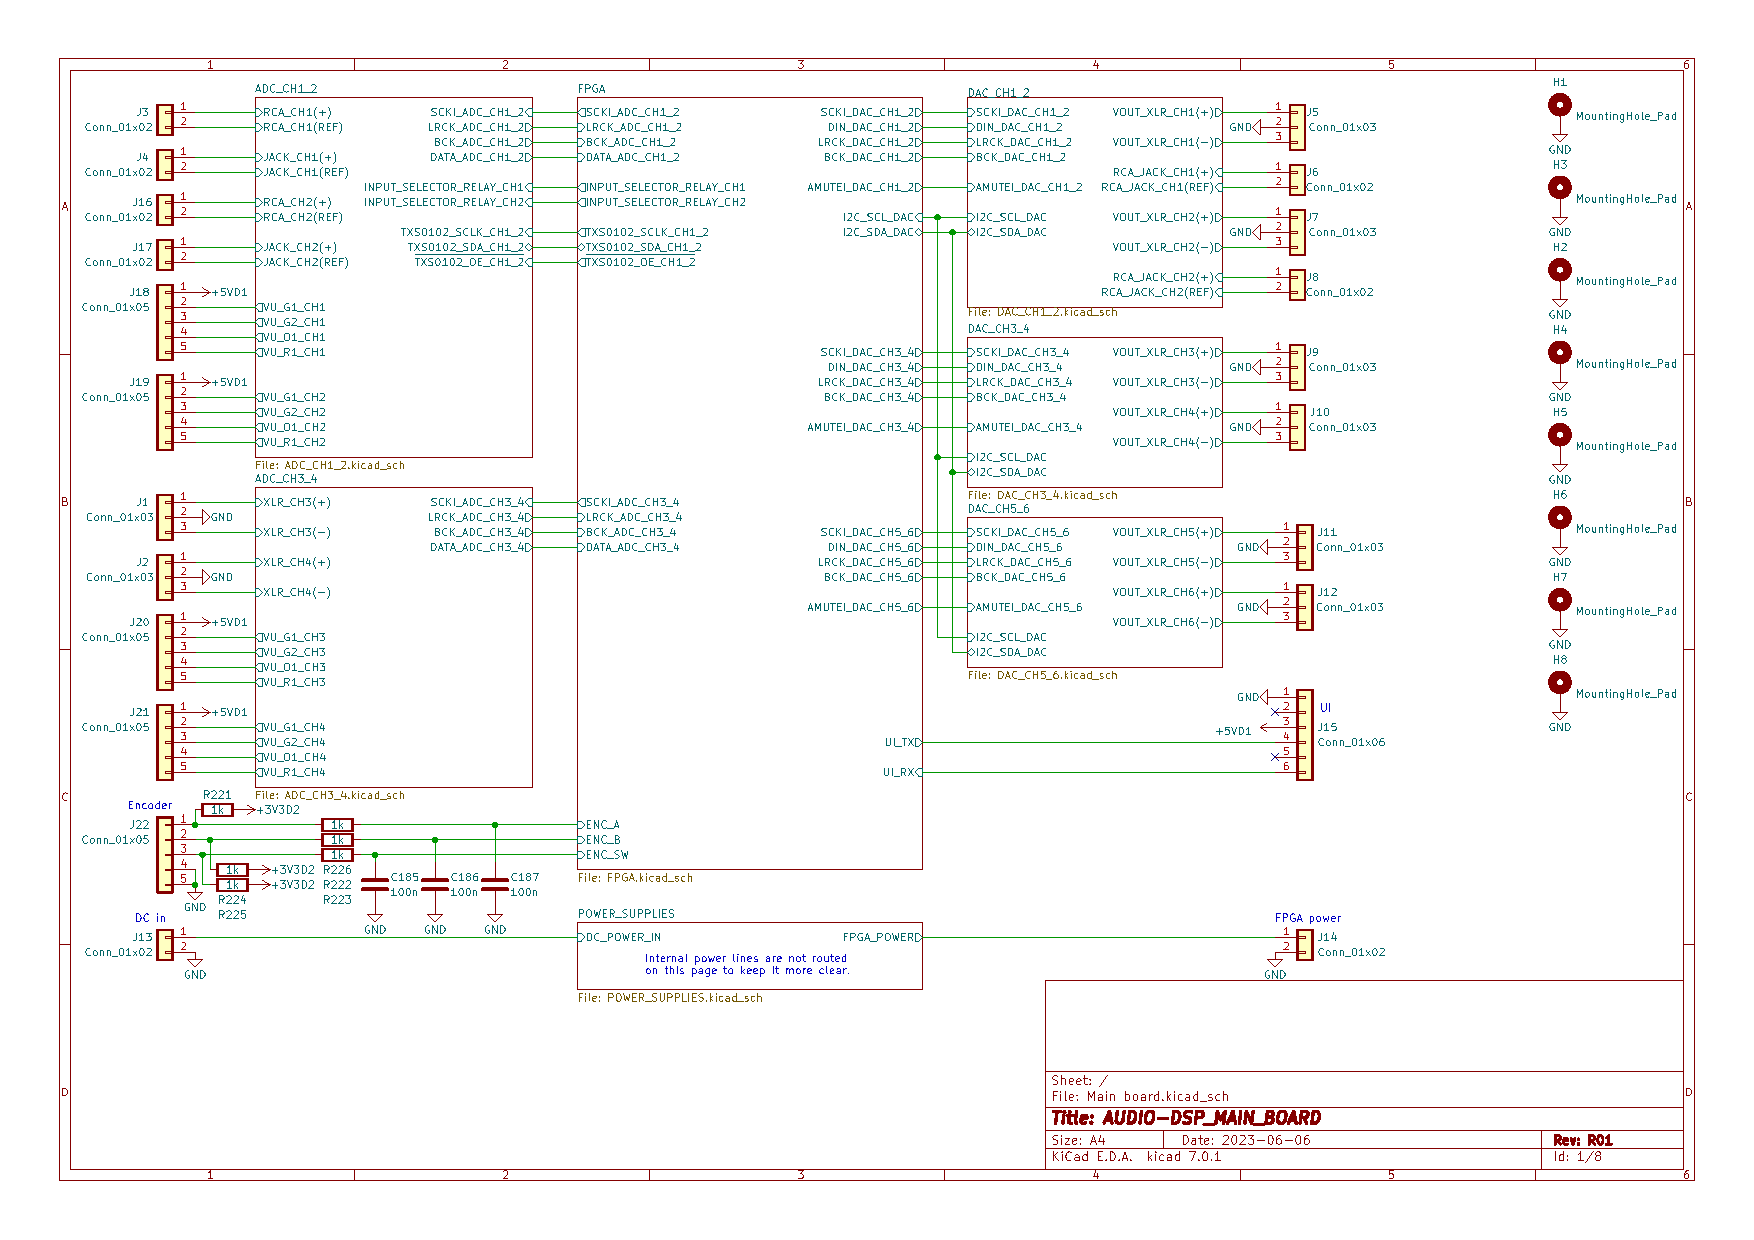
\includepdf[angle=90, pages=-]{Main_board_schematic.pdf}

\section*{Appendix C: Buck converter schematic}
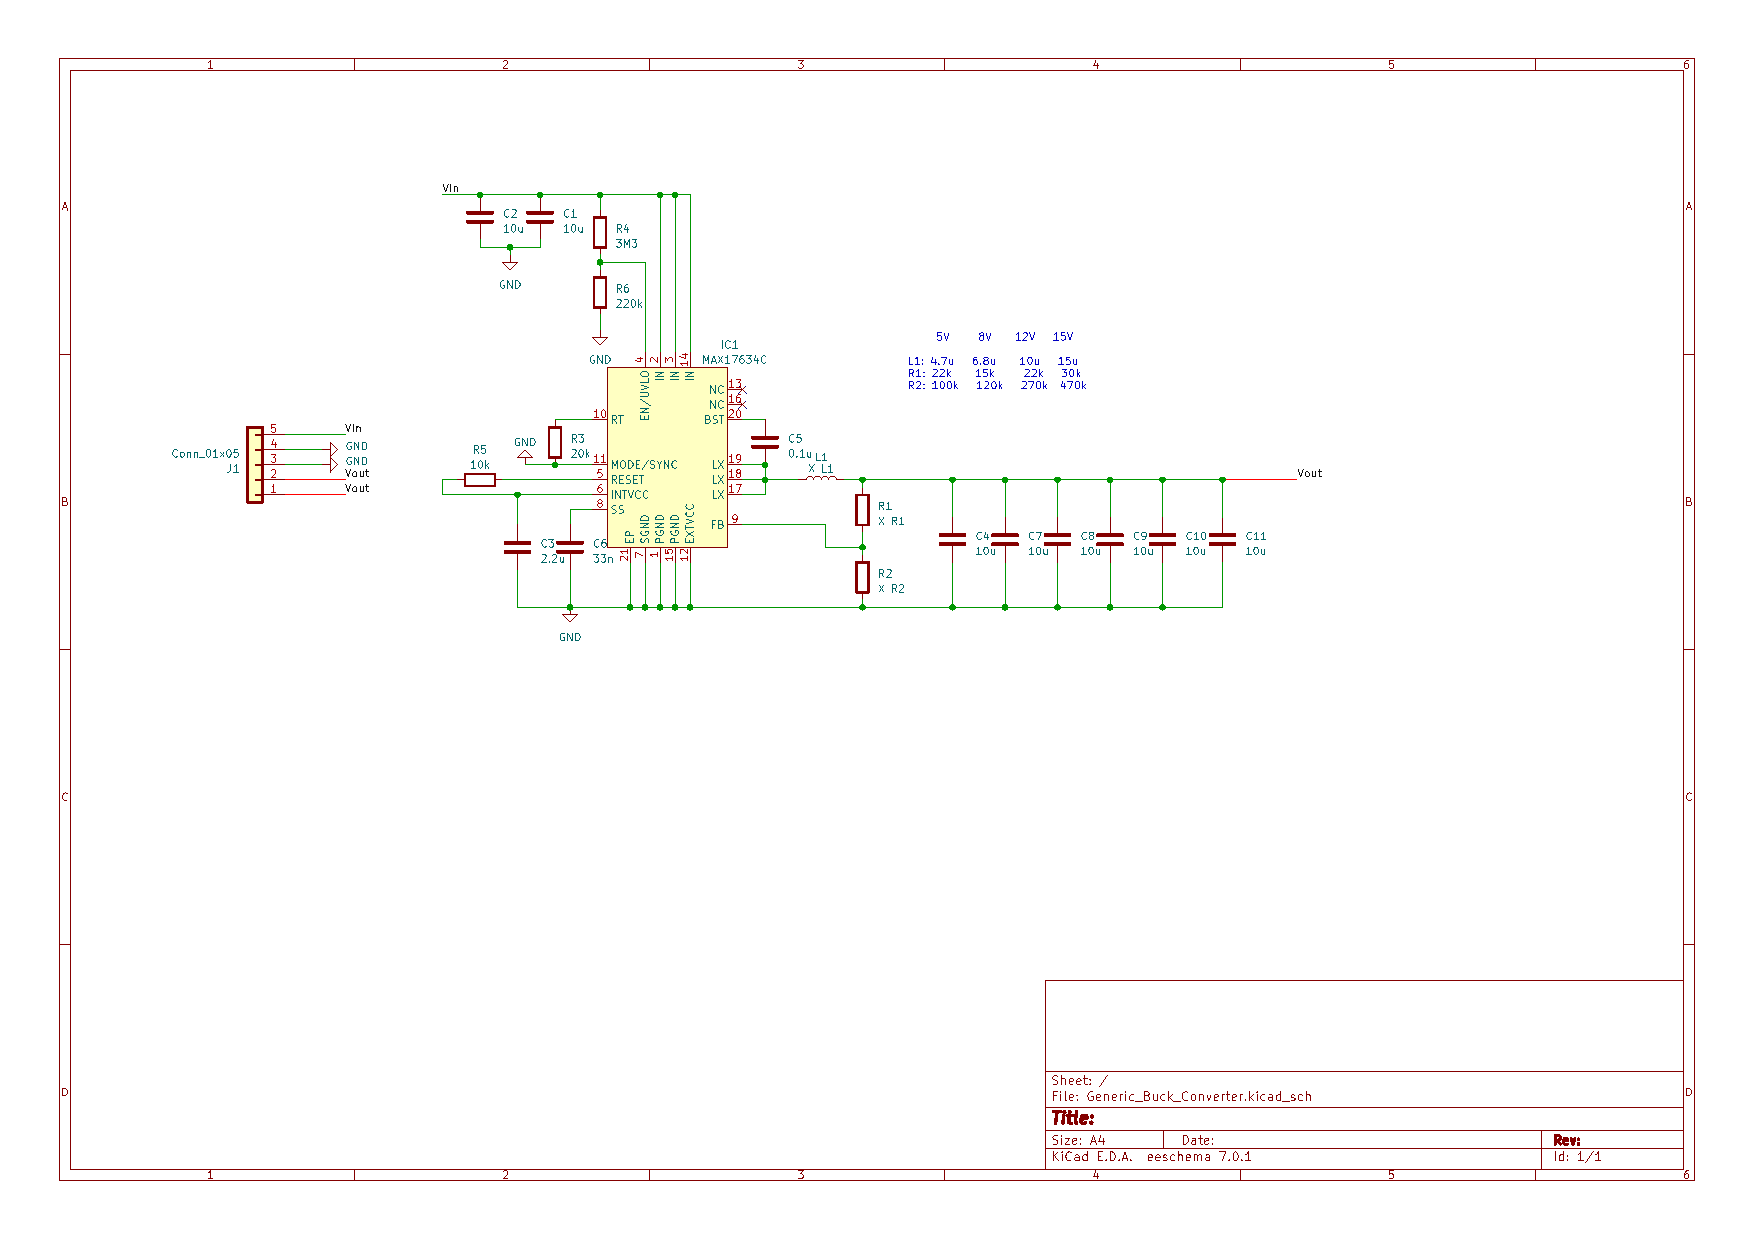
\includegraphics[angle=90, width=500pt]{Generic_Buck_Converter_schematic.pdf}

\section*{Appendix D: Linear regulator schematic}
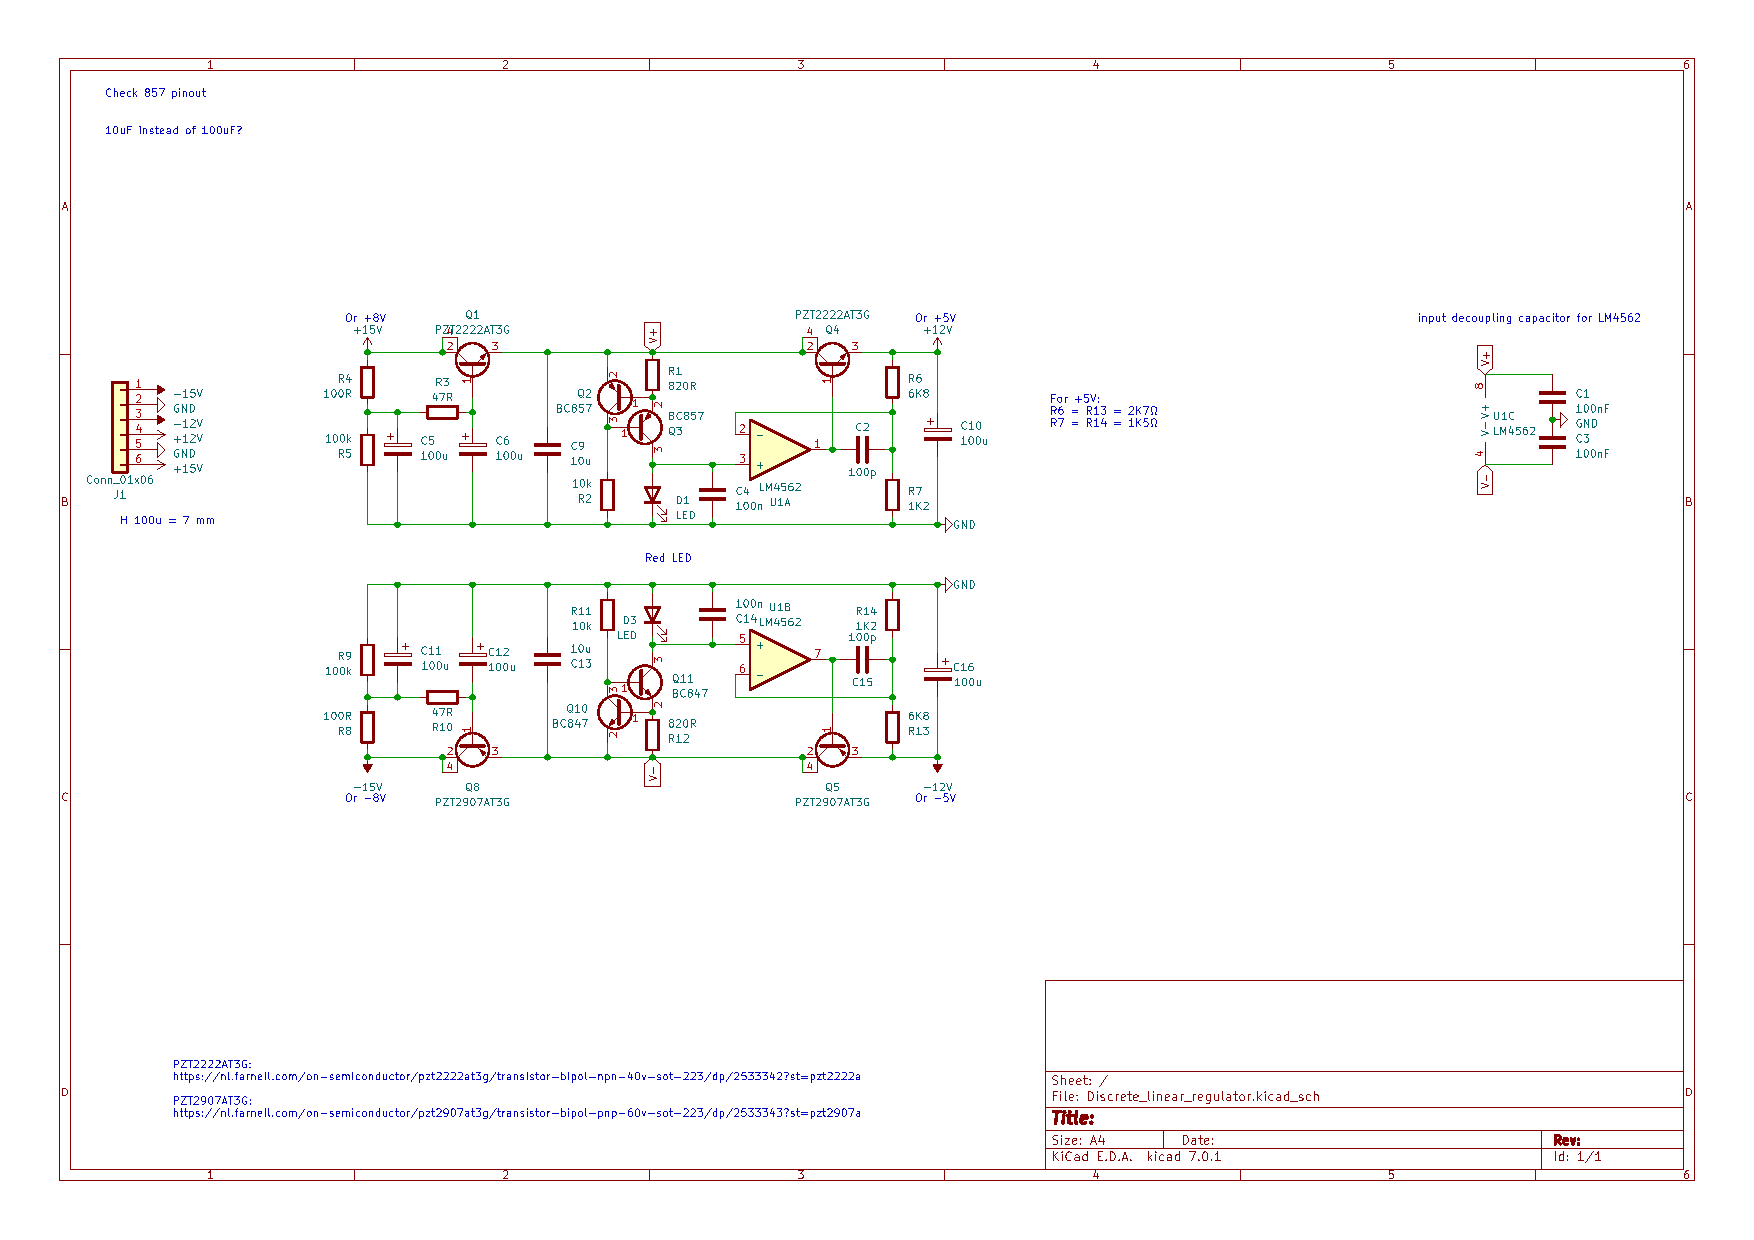
\includegraphics[angle=90, width=500pt]{Discrete_linear_regulator_schematic.pdf}

\section*{Appendix E: SEPIC schematic}
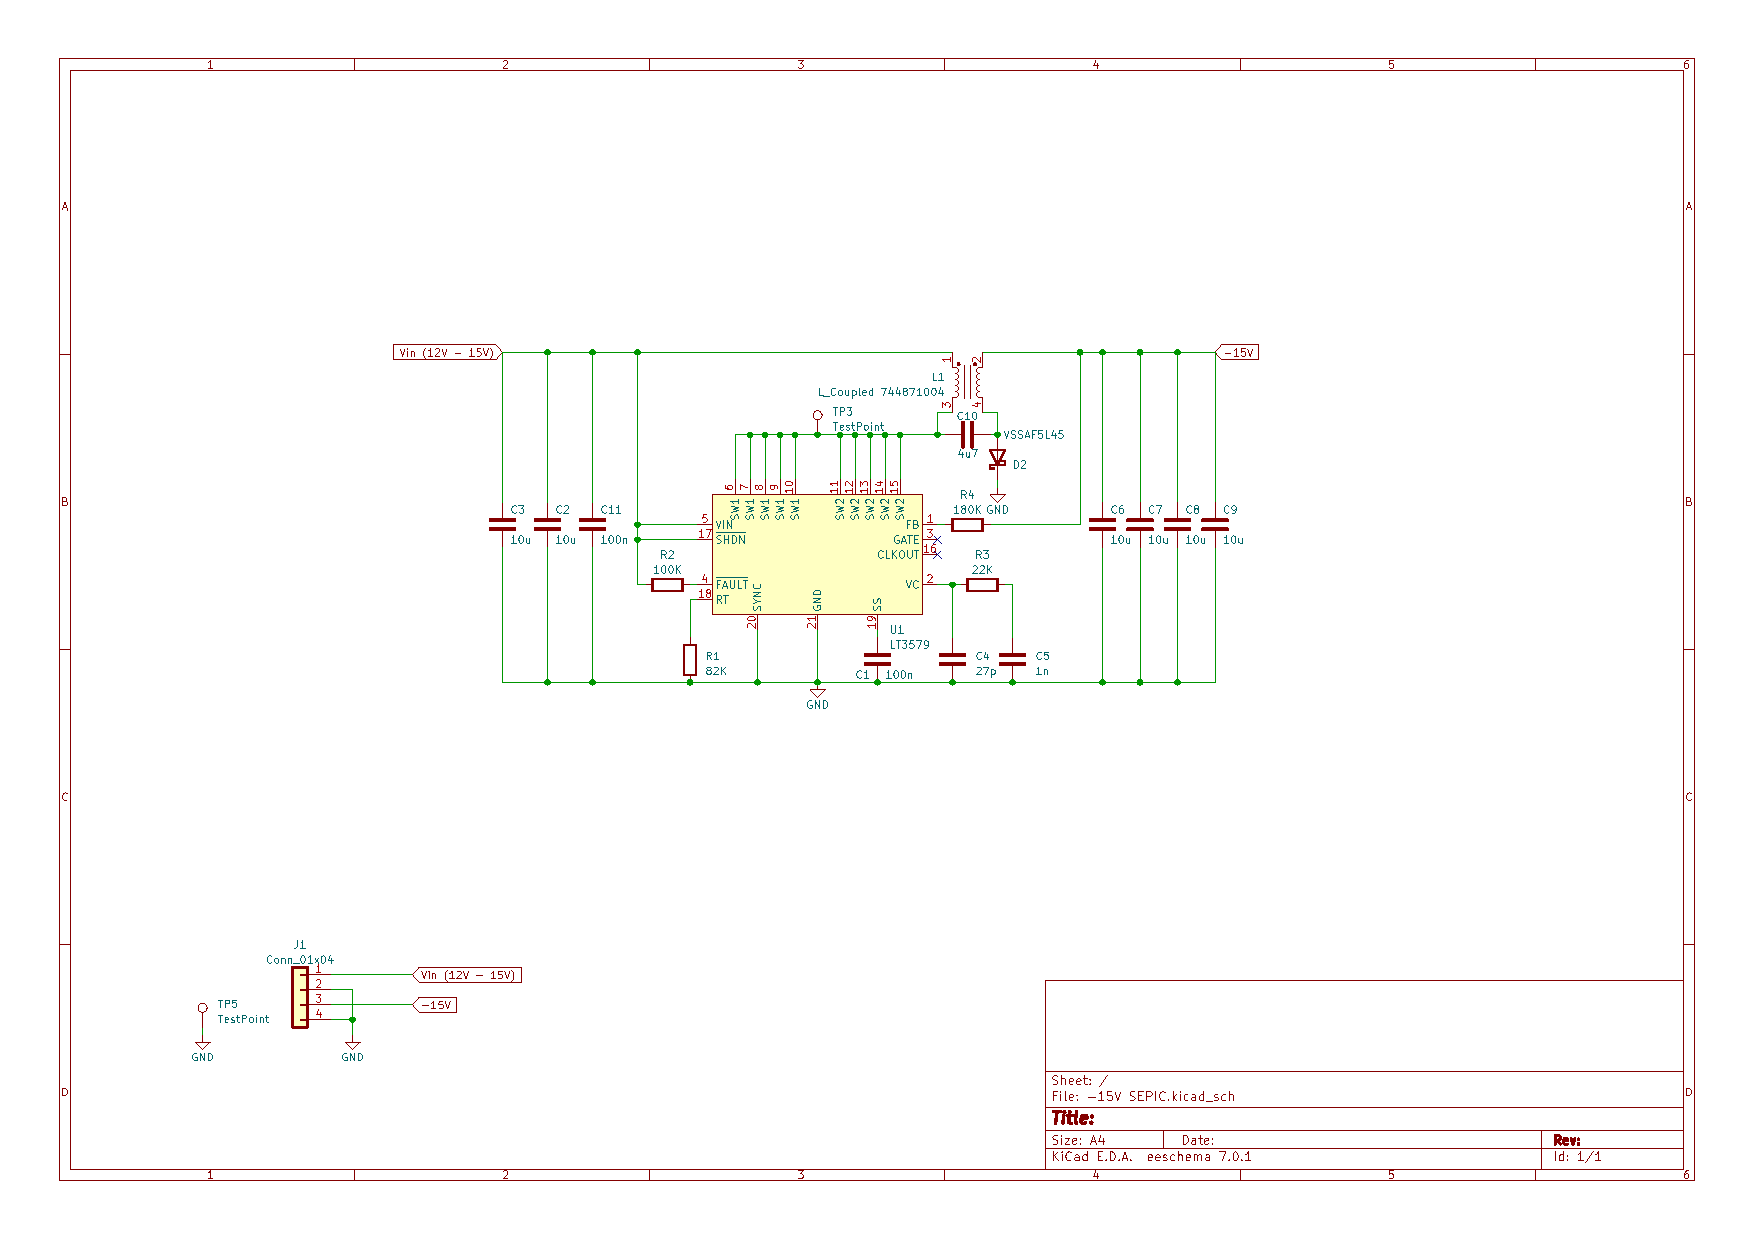
\includegraphics[angle=90, width=500pt]{-15V_SEPIC_schematic.pdf}